\documentclass[paper=a4, fontsize=10pt]{jlreq}

\usepackage{amsmath, amssymb}
\usepackage{enumerate}
\usepackage{tikz}
\usepackage{listings, xcolor}
\usepackage{graphicx}

\lstset{
  basicstyle = {\ttfamily},
  frame = {tbrl},
  breaklines = true,
  numbers = left,
  showspaces = false,
  showstringspaces = false,
  showtabs = false,
  keywordstyle = \color{blue},
  commentstyle = {\color[HTML]{1AB91A}},
  identifierstyle = \color{black},
  stringstyle = \color{brown},
  captionpos = t
}

\title{情報学群実験第3 NetworkSimulator}
\author{学籍番号 1280391 \\ 細川 夏風}
\date{\today}

\begin{document}

\maketitle
\section{実験内容}
\subsection{実験A}
帯域幅を$1, 2, 3, 4, 5, 9, 18$\texttt{Mbps}の順番に変化させ，その帯域幅の輻輳ウィンドウサイズ(\texttt{cwnd})とスロースタート閾値(\texttt{ssthresh})の時間の関係の変化をグラフに図示する．また，スループットのついても理論値と実測値で解析を行う．
\subsection{実験B}
帯域幅を$5 \sim 25$\texttt{Mbps}まで$5$\texttt{Mbps}ずつ変化させ，グラフに図示する．その際のスループットの飽和についてグラフから考える． 

\section{実験方法}
\subsection{実験A}
実験Aでは以下のシェルスクリプトを用いてシミュレーションを実行した．

\lstinputlisting[language=bash, caption=kadai2-2-A.sh]{kadai2-2-A/kadai2-2-A.sh}

\subsection{実験B}
実験Bでは以下のシェルスクリプトを用いてシミュレーションを実行した．

\lstinputlisting[language=bash, caption=kadai2-2-B.sh]{kadai2-2-B/kadai2-2-B.sh}

\newpage

\section{実験結果}
\subsection{実験A}

\newcommand{\bwfig}[1]{%
  \begin{figure}[htbp]
    \centering
    \begin{minipage}[b]{0.48\linewidth}
      \centering
      \includegraphics[width=\linewidth]{kadai2-2-A/result_BW#1_cwnd_max.pdf}
      \par\smallskip(a) cwnd\_max
    \end{minipage}
    \hfill
    \begin{minipage}[b]{0.48\linewidth}
      \centering
      \includegraphics[width=\linewidth]{kadai2-2-A/result_BW#1_cwnd_ssthresh.pdf}
      \par\smallskip(b) cwnd\_ssthresh
    \end{minipage}
    \caption{帯域幅 #1\,Mbps における cwnd および ssthresh の時間変化}
  \end{figure}
}

\bwfig{1}
\bwfig{2}
\bwfig{3}
\bwfig{4}
\bwfig{5}
\bwfig{9}
\bwfig{18}

\newpage

\subsection{実験B}
\begin{figure}[htbp]
  \centering
  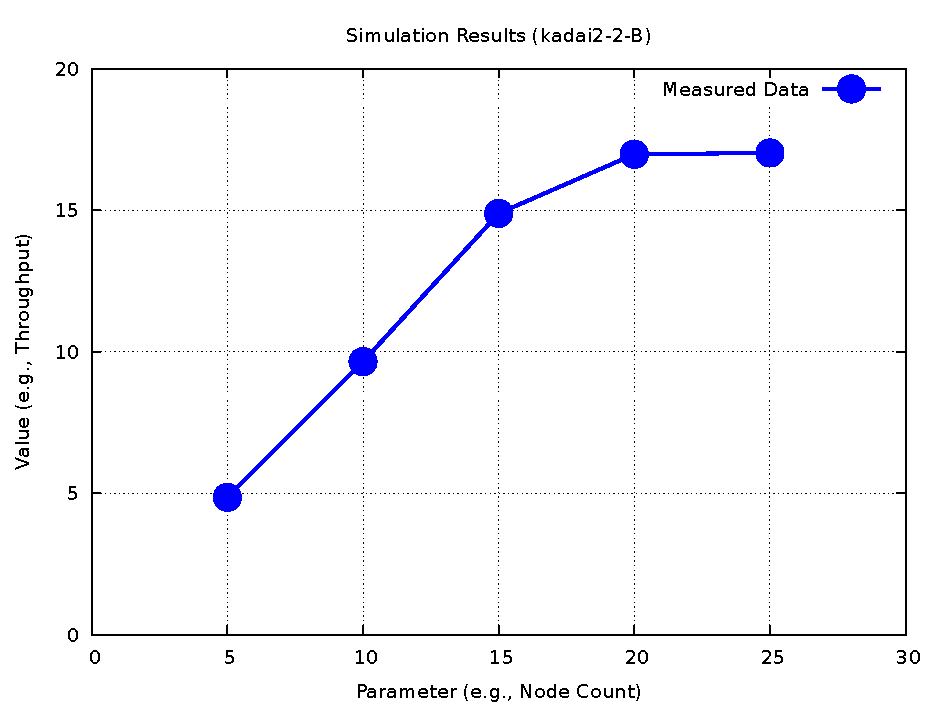
\includegraphics[width=0.75\linewidth]{kadai2-2-B/kadai2-2-B_plot.pdf}
  \caption{帯域幅とスループットの関係}
  \label{fig:exp_B}
\end{figure}

\section{考察}
\subsection{実験A}
以上の図から以下の事がわかる．パケットの損失が起きる頻度は帯域幅が増加するにつれて多くなっている．しかし，ある帯域幅以上になるとパケットの損失は減っている．これは帯域幅が小さい状態はパケットの輻輳制御がしっかりと作動していることが理由であると考えられる．その理由に\texttt{ssthresh}の値がわずかに小さいことが図から読み取れる．また，\texttt{cwnd}の値の増加率が帯域幅の増加に合わせて大きくなっていっていることがわかる．しかし，ある帯域幅からパケットの損失が極端に減るか，確認されない．これは送信しているパケットのデータ量に比べて帯域幅が十分に大きくなったことが理由であると考えられる．

\subsection{実験B}
図\ref{fig:exp_B}から，スループットの上昇率が非常に低くなっているか限りなく$0$\% に近い状態となっていることがわかる．これは前述の通り，送信するデータ量に対して帯域幅が十分に大きくなったため，パケットの損失率が減ったためであると考えられる．

\begin{thebibliography}{99}
  \bibitem{}
\end{thebibliography}

\end{document}
